\section{Introduction}
\label{sec:introduction}

SARS-CoV-2 (COVID-19) has changed the landscape of the world today. 
On March 11,2020 it was declared a global pandemic, threatening many lives globally. Scientists have been racing to not only develop a vaccine, but also construct accurate evolutionary diagrams. 
Therefore the field of phylogenetics has been crucial in tracking the relationships back to its origin. 
Though its origin still remains ambiguous, scientists have been able to track some of their closely-related evolutions using a series of alignment techniques to find small differences between genomes. 
Of the many representations, \emph{phylogenetic time trees} are the focus of this research. 
Being seen as an evolutionary time map, we can see a small depiction of its evolution relative to time. 
Mathematically we can also visualize them as a dynamical system. 

\begin{figure}[h]
\centering
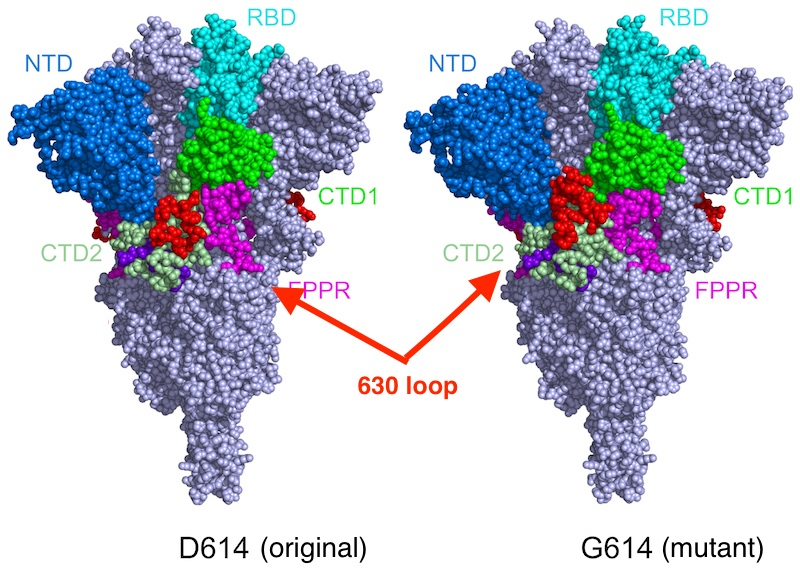
\includegraphics[width=.45\textwidth]{figures/Cov2.jpg}
\caption{\textbf{Pictured}: SARS-CoV-2 Spike protein structure, Delta Variant Spike protein structure \cite{Fliesler}}
\end{figure}

Our species of interest is not the coronavirus, but a subcategory of it. 
The Deltacoronavirus variant was first reported in India in late 2020 and has been spreading widely across the USA. 
Unlike the original virus, the delta variant is proven to be more contagious. 
Due to a slight change in its structure as seen in \textbf{Figure 1}, this has changed how the virus interacts with our cells. 
Once this variant comes into contact with a host receptor, it is actually better in terms of efficiency and at infecting them. 
For this reason the transmission of this particular virus has been widespread. 
And because of its current relevancy, we have chosen to use this species to model for our representation of the phylogenetic time tree.        

\section{Genetic Algorithm}

The Genetic Algorithm (GA), is a metaheuristic algorithm inspired by Charles Darwin's theory of Natural Selection. 
This machine learning algorithm uses three components (Fitness, Single-Point Crossovers, Mutations) and is primarily used to solve optimization problems. 
With this method being stochastic meaning, it relies on randomness, our solutions do not have a definitive outcomes and are solely approximations. 
Our reasoning to choose this specific methodology is due to its performance in navigating massive search spaces. 
With our intentions to work with 112 different delta variant genomes, we need to consider the overwhelming number of combinations there are to construct our tree. 
Governed by the equation below we plug in $n = 112$ to resemble the amount of genomes used in this research:

\begin{equation}
\label{Combinations}
\frac{(2(n)-3)!}{2^{n-3}(n-3)!}
\end{equation}

\begin{equation}
\label{Combinations2}
\frac{(221)!}{2^{109}(109)!}
\end{equation}

\begin{equation}
\label{Combinations3}
\frac{5.047331342371357620848E423}{6.490371073168534535663E32(1.443859583202493582205E176)} = 5.386012149439842115461E214
\end{equation}

As seen in Equations 1,2,3 the following computation shows the amount of different combinations in which we could construct this tree. 
And as expected it is exceedingly overwhelming. 
Therefore machine learning algorithms like the GA have features like backwards propogation, and gradient descent that allow these solutions to learn the context of their data and provide better solutions as a result. 
With computation allowing us to be able to solve these massive combinatorics problems, this field is at the brinks of its capabilities. 
Regardless, the GA is a novel approach in solving these problems and we wish to use its output data to construct our trees. 
Below in \textbf{Figure 2} is a flowchart of how the processes within the algorithm all work together. 
These components will be explained in greater detail in the coming sections.

\begin{figure}[h]
\centering
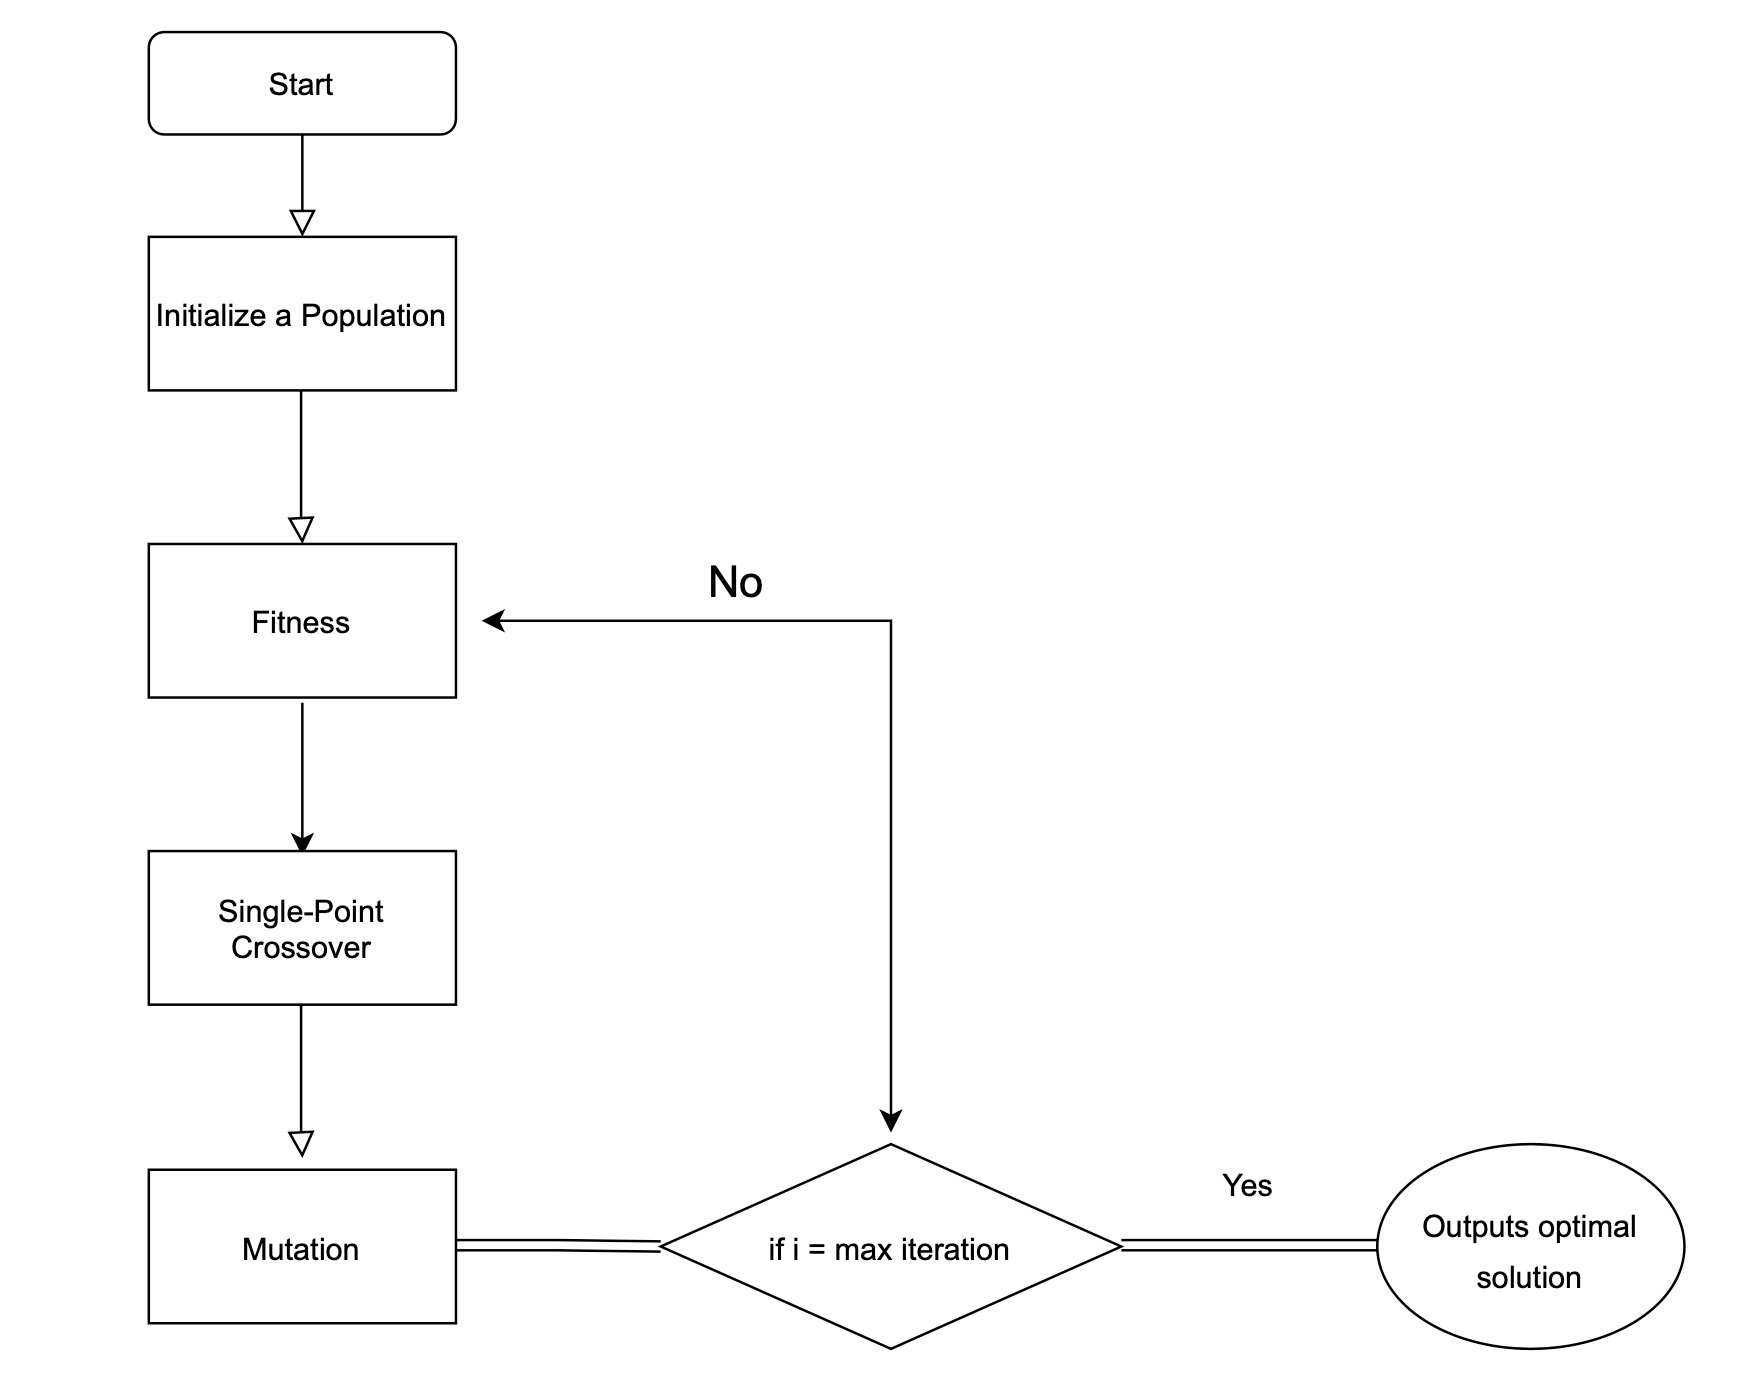
\includegraphics[width=.5\textwidth]{figures/flowchart_GA}
\caption{Flowchart of the Genetic Algorithm}
\end{figure}
  
\subsection{Fitness}

"Survival of the Fittest" is a commonly used phrase in evolutionary biology to express how only the selected best solutions/species will make it to the next generation. 
As a result, we need to implement a similar implementation into our algorithm which evaluates how well a solution is. 
With our objective to line up these genomes based on how similar they are from one to another, our Genetic algorithm is assessing fitness based on how the sequence is lined up. 
Overtime these solutions should slowly begin to rearrange themselves in an order that embodies that of the distance matrix we intend to use. 
Visually we can see this improvement as seen in \textbf{Figure 3}. 

\begin{figure}[h]
\centering
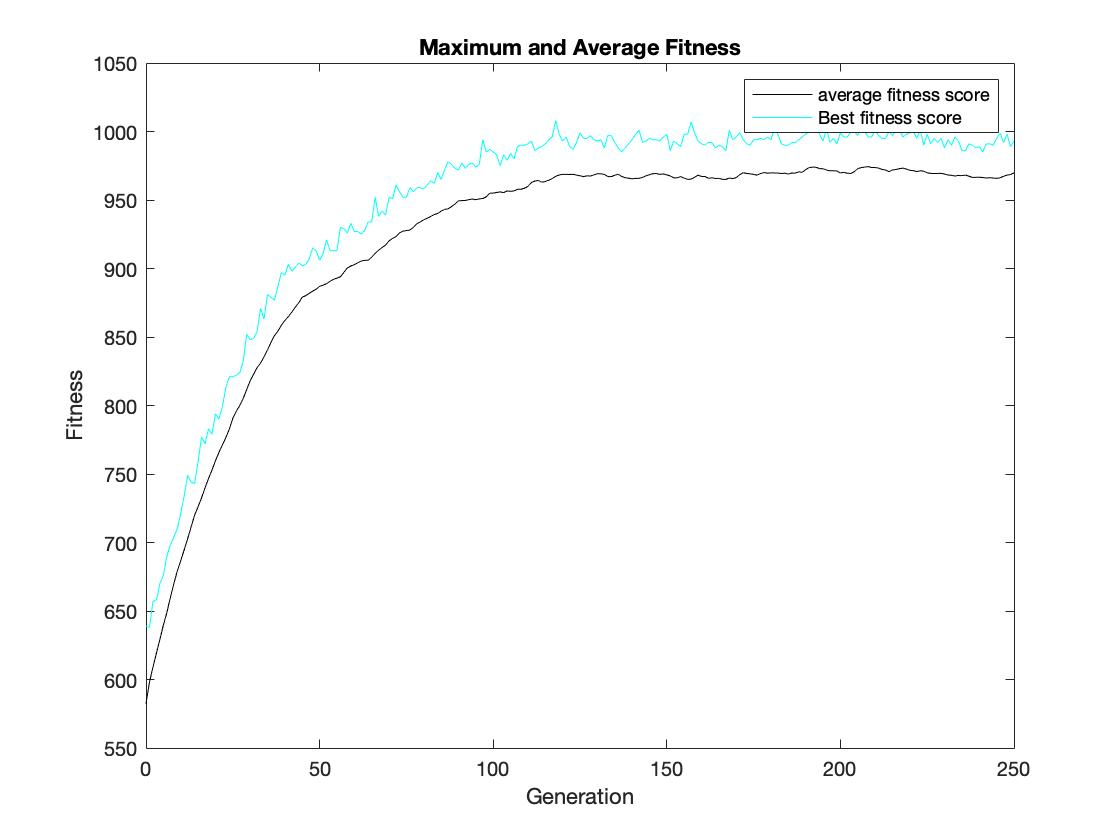
\includegraphics[width=.75\textwidth]{figures/Fitness.jpg}
\caption{Graph that shows the improved fitness over a series of 250 iterations}
\end{figure}

\subsection{Single-Point Crossovers}

The second part of this algorithm involves how these solutions actually gain a higher fitness score. 
The only way to continue to have improved results is to perform a reproduction method known as the \emph{single-point crossover}. 
In evolutionary biology, gene conversion can be \emph{allelic}, meaning that one allele of the same gene replaces another allele from another gene. 
Similarly in this function, we perform a swap of a random number of genomes $1 \leq x \leq$ (number of genomes - 1). 
This will then swap a portion of the two randomly selected solutions and create a new solution whose order is closer to that of an optimal solution. 
These two newly generated solutions begin what would be the next generation. 
We repeat this process as long as there are remaining genomes from the past generation. 

However, this algorithm unfortunately is not perfect because our single-point crossover and selection functions are governed by randomness. 
The reason randomness is an issue is because there is no way to guarantee that we won't destroy our best solutions produced from each preceding generation. To resolve this issue, we must introduce a process called \emph{elitism} \cite{Ahn}. 
Elitism can be described as, the most fit handful of solutions are guaranteed a place in the next generation - without undergoing mutation. 
So, in order to preserve the most fit solutions, we must select the top 10 genomes whose contents will be copied into is successive generation. 

\subsection{Mutation}

The last component as alluded to in the previous section is mutation. 
Mutations in evolutionary biology are simply a change in a sequence of an organism's DNA. 
However, since we are not working with nucleotide bases but rather with genome order, we must also familiarize ourselves with \emph{noise}, a concept that dates back to an interests of Einstein (1905). 
In the communication domain, noise (unwanted random disturbances) make it difficult to have a trivial signal. 
These fluctuations occur when there is a suspected origin that implicates the action of a very large number of "degrees of freedom" or variables. 
The coupling of noise to nonlinear systems can lead to non-trivial effects like, unstable equilibria and shift bifuracations \cite{Gammaitoni}. 
Therefore it is widely believed that noise drastically modifies the deterministic dynamics of this system adopting its stochastic qualities. 
So in our case, noise behaves similarly to mutations where a singular random genomes might get flipped. 
The way we simulate this behavior on a computer is by random probability. 
Though it may be possible to destroy one of our best solutions, mutations are essential to evolution. 
With that being said although there is some random probability to destroy our best fit solution, there is also an equal chance that we construct an even better one. 

\subsection{Loss Function}

Now that the algorithm's components are understood, we can also explain the calculus behind the machine learning. 
A \emph{Loss Function} is what governs the learning of a machine. 
Its a method of evaluating how well the algorithm performs given some set of data.
And in optimizations we are seeking to find the minimums of these loss functions.
However, there are ways to improve the overall accuracy of the predicitions.
Therefore, \emph{Backwards Propogation}, is a mathematical tool for improving the accuracy of predictions in machine learning. 
As we saw in \textbf{Figure 3}, the algorithm slowly begins to pick up on accuracy at a rapid pace, even though it is a stochastic. 
Primarily in optimizations, finding the minimum or the local minima of a function can tell you the minimal cost of a particular function. 
In fact mathematically this is exactly what we are looking for. 
But the issues that arise is how we could have this algorithm learn to make decisions based on the data they are presented. 

In vector calculus there is a concept called the \emph{gradient} $ (\nabla) $, which will essentially provide the slope of a tangent plane to indicate how deep it is. 
This information is particularly useful to us because if we take the negative of the gradient of some cost function C, $ -\nabla (C) $ \cite{BB}, we will begin to know which direction to move along the plane. 
So as long as the negative of the gradient is being taken, we will continue to move towards the local minima of a xyz plane. 
This process is what we call \emph{The Gradient Descent}. 
However if we refer back to \textbf{Figure 3}, we will notice that the curve will begin to plateau and sort of oscillate around this most fit region. 
The reason this occurs is due to the characteristics of this stochastic algorithm. 
Even when the algorithm obtains their "most optimal" solution, it does not know that it is the best until all the iterations have concluded. 
And since the single-point crossovers occur every generation, these "most optimal" solutions get altered. 
Therefore a better representation of our algorithm will appear as a \emph{stochastic gradient descent}. 
These two concepts are pictured in \textbf{Figure 4}.   

\begin{figure}[h]
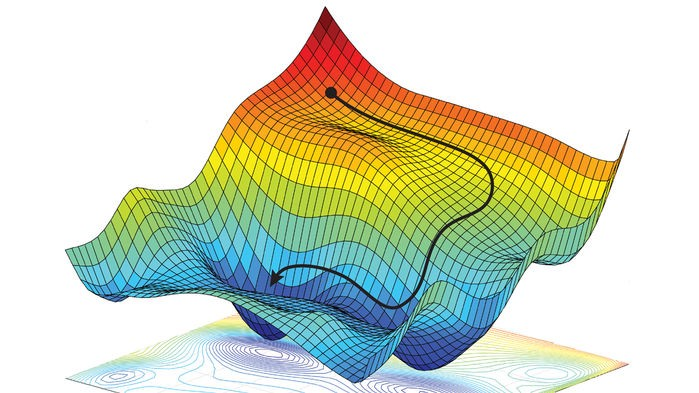
\includegraphics[width=.5\textwidth]{figures/bp.jpg}
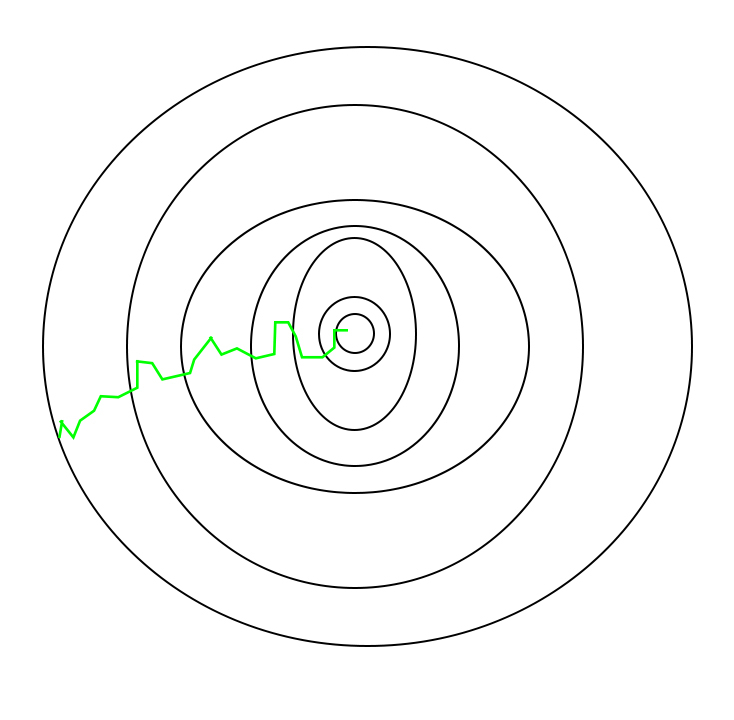
\includegraphics[width=.35\textwidth]{figures/sgd-1.jpg}
\caption{Gradient Descent in a xyz plane, Stochastic Gradient Descent in a depth map}
\end{figure}   

\section{Phylogenetics}

Phylogenetics is the study of evolutionary relationships among biological species. The similarities in biological function and molecular mechanisms in these species or \emph{taxa} suggests that species come from a shared ancestor. This method has been used by bioinformaticians, to identify disease causing microbes, and determine its origin, how it might have spread, and routes of transmissions. As a result modeling the Delatcoronavirus variant should be no different and we wish to model an evolutionary tree with respects to time. In this temporal framework, time flows from the roots to the tips. And to completely understand the architecture of these trees we also need to introduce a little bit of graph theory. 

\begin{figure}[h]
\centering
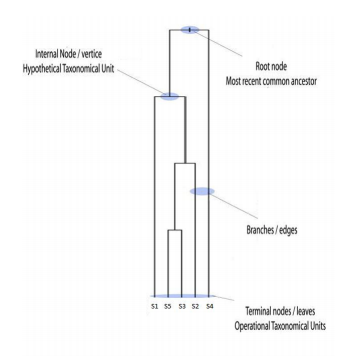
\includegraphics[width=.5\textwidth]{figures/ptrep.png}
\caption{The phylogenetic tree structure diagram}
\end{figure}

The basic components of a phylogenetic tree as represented by \textbf{Figure 5}, contains branches, also called edges that are connected to and terminate nodes or vertices. Branches can be classified in one of two ways: internal or external (terminal). These terminal nodes that are found at the tips of trees represent \emph{operational taxonomic units} also reffered to as OTU's. The essence of an OTU is to correspond their molecular sequences or species (taxa) from which the tree is deduced. Conversely, internal nodes represent the last common ancestor to the nodes that arise from the that point. The type of tree, we intend to work with is composed of a multi-gene family called a gene tree which looks at one species and all its different variations.

\begin{figure}[h]
\centering
\includegraphics[width=.35\textwidth]{figures/clade.pdf}
\caption{The distinctions of what is a clade and what is not a clade}
\end{figure}   

On top of the basic components of a tree we also introduce a \emph{clade}. Clades which will appear frequently are structures of organisms that includes a single ancestor and all of its descendents \cite{Clade}. Also called monophyletic groups, these represent unbroken lines of descent. An easy way to visualize this concept is to clip any single branch off a tree. All the descendants on that branch is considered to be apart of that clade. If for whatever reason, there needs to be a cut made from a separate group from the rest of the tree, that group does not form a clade. Such non-clade groups are called polyphyletic. A visualization of this concept can be seen in \textbf{Figure 6}. 

\subsection{NP-hard Problems}

Finding the most fit tree (solution) under any criterion, is considered to be a NP-hard problem within phylogenetic trees. 
In computer science there remains an unsolved hypothesis known as the \emph{P versus NP problem} \cite{Hardesty}.
Computer Scientists typically like to ask "How long will it take to execute a given algorithm?"
However, instead of expressing it in minutes, seconds, they give an answer relative to the number of elements the algorithm has to manipulate.
As we expressed in \textbf{Section 2}, the amount of different combinations it has to go through is an overwhelming 5.386012149439842115461E214.
This would obviously take a lot of time to solve, and therefore has properties of an NP-hard problem. 
Another way to look at this problem is to determine whether every problem whose solutions can be quickly verified, can also be quickly solved for. 
P stands for polynomial time, which roughly means a set of relatively easy problems to be solved for. 
NP stands for non-deterministic polynomial time which is a set of difficult problems to be solved for. 
So, if P = NP , this would imply that the difficult set of problems have relatively easily computed solutions.

While the hypothesis has yet to be proven, computation has been a powerful tool capable of solving NP-hard problems. 
With machine learning having a much larger presence in the way we analyze data, we could use a metaheuristics like the GA to approach these problems.
So being able to solve problems that we thought could not be solved in a lifetime has opened up a new area of research and researchers are just scratching the surface in solving  NP-hard problems.   
This research aims to solve the phylogenetic tree construction, a NP-hard problem in bioinformatics, using the GA as our focal study. 
The two approaches we use are the \emph{Distance Matrix}, to provide instructions on how to build the tree and the \emph{Neighbor-Joining Algorithm} which builds the tree itself.  

\subsection{Dynamical Systems}

In mathematics, a \emph{dynamical system} is a system in which a function describes the time dependence of a point in a geometrical state space. The evolution rule of the dynamical system is a function that describes what future states follow from the current state. In our case we are working with a completely stochastic system, in which random events affect the evolution of the geometric manifold. This field of study has wide applications in many biological sciences, and to an extent the phylogenetic tree is a representation of a dynamical system. Because our focus is the phylogenetic time tree the branch lengths actually have a correspondence to time. We will explore the two methods (The Distance Matrix Approach, and Neighbor-Joining Algorithms) in the coming sections and what maths are applied within these components. But before doing so, we must introduce a big aspect of phylogenetics which is analyzing the bifurcations that occur within these trees.

Phylogenetic inferences are depicted in the form of a hierachical bifurcation tree. Bifurcations, which are a series of branching processes, have one branch line and it is split into two descendents. \cite{Ecology} Therefore positioning of organisms on these trees rely solely on their genetic similarity between each other. Distance methods like the ones used in this research are based on measures of evolutionary distinctiveness between all pairs of taxa. So if we are analyzing 112 Deltacoronvirus variant genomes, there is no guarantee that all these genomes have some shared ancestor amongst each other. So while bifurcations are simple splits that occur in a tree, we may also see \emph{outgroups}. An outgroup is a lineage that falls outside the clade being studied but is still closely related. \cite{Clade} These metrics are calculated based on differences of nucleotides from DNA sequence data (provided by the NBCI). In our approach this distance method is taken care of by the GA, which learns to find the similarities and constructs an approximation with the data it is provided. We now proceed to explaining our planned methodologies to build our trees.    

\subsection{The Distance Matrix}

Our preferred method of choice and the focus of this paper will be on the \emph{Distance-matrix Method}. 
Distance-matrix methods are far more rapid compared to popular methods like the  \emph{maximum-likelihood}, and it essentially measures the genetic distances between sequences. 
Once these distances are found, a distance matrix will be constructed, where the distance equates to the approximate evolutionary distance. 
However, the challenging aspect of this computational method is constructing the matrix itself. 
The distance matrix can be visualized as a $n * n$ matrix, where \emph{n} resembles the number of sequences. 
Every row corresponds to a single sequence and every columns corresponds to the distance between the sequences. 
By getting some collection of $n$ sequences, the matrix below can be constructed:

\begin{equation}
\label{Distance-matirx}
\begin{bmatrix} 
d_{11} & \cdots & d_{1n} \\
d_{21} & d_{22} & d_{2n}\\
\vdots & \ddots & \vdots\\
d_{n1} & \cdots & d_{nn} \\
\end{bmatrix}
\end{equation}       
In the distance matrix above, $d_{ij}$ can be broken down to where the distance is measured between the $i_{th}$ and $j_{th}$ sequences. 
Though this measure of weight is up to choice with methods like \emph{Jukes-Canton and p-Distances}, we are going to be using a Genetic Algorithm, to find out the particular order. 
This method will be used to obtain the genetic distance from a its machine learning to help us construct our distance matrix which will then be fed into the neighbor-joining algorithm. 
Using this algorithm we will compute an unresolved star tree topology, and transforms it into a tree where all the branches lengths (time) are known. 
This method relies solely on how the matrix is constructed because there are a number of combinations that can be constructed within the distance matrices to feed the algorithm.      
 
Distance-based methods like the neighbor-joining algorithm, are polynomial time and are quite rapid in practice. 
Within the distance-based methods, there are two different algorithms: \emph{cluster-based} and \emph{optimality-based}. 
The cluster-based algorithm builds its distance matrix by starting at similar sequence pairs, which are then used to construct the tree. 
This algorithm is found within the \emph{UPGMA} or \emph{unweighted pair group method using arithmetic average}, and our \emph{neighbor joining}. 
Meanwhile the optimality-based algorithm compare multitudes of different tree topologies and selects the best fit by determining computing distances in the trees, and the desired evolution or \emph{actual evolutionary distance}. 
This algorithm is common in \emph{Fitch-Margoliash} and \emph{minimum evolution} methods. 
But in retrospect, both these algorithms are computationally simpler than a maximum likliehood which is the conventional method used to approach these problems.
However, since our interest is based on computational speed, we prefer this distance-matrix method over this conventional model.  

\subsection{Neighbor-Joining Algorithm}

\begin{figure}[h!]
\centering
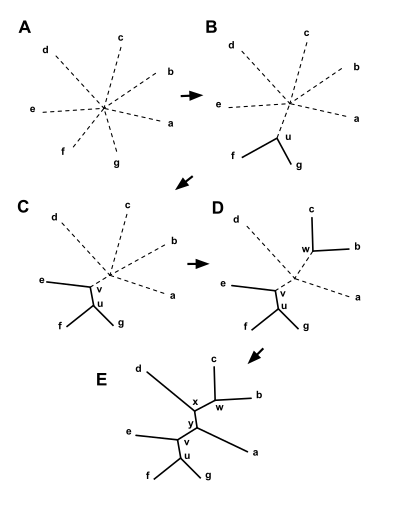
\includegraphics[width=.35\textwidth]{figures/nj.png}
\caption{A visual representation of a distance matrix containing 7 species, beginning in the star-shape which then is then slowly constructed into a tree using the neighbor-joining algorithm based off a specific distance-matrix}
\end{figure}

Now that we have obtained a distance matrix, we can begin to construct the trees. As described in \textbf{Figure 7}, the tree begins in a star formation where there is no tree or lengths of branches shown or combined into internal nodes. But with this distance matrix, the distances represent the dissimilarity of the aligned sequence and can begin subsequent joining between neighbors. So from the diagram we can see that each OTU is represented as a fork. For each OTU, you want to compute the sum of distance between OTU one and another OTU, divided by (N-2), where N is the total number of OTU's. The equation can be represented to describe the following: 

\begin{equation}
\label{computation}
S_i=\frac{1}{N-2}\sum_{k=1}^{N} D_{ik}\\
\end{equation}
Once you combine the two taxa on a node into a sub-tree, you want to calculate the new branch length which can be calculated by the following equation:

\begin{equation}
\label{branch-length}
D_{Xi} = \frac{D_{ij}+S_i-S_j}{2}, D_{Xj} = \frac{D_{ij}+S_j-S_i}{2}\\
\end{equation}
And at last calculating the new matrix distance is done by connecting $i$ and $j$ and replace it with a node $x$ that connects it to the final equation:

\begin{equation}
\label{branch-length}
D_{xk}=\frac{D_{ik}+D_{jk}-D_{ij}}{2}\\
\end{equation}
This sequence of steps are repeated for (N-2)! iterations. This mathematical algorithm is what gives the layers within the trees. After combining similar trees to each other, the matrix size begins to become smaller and smaller and the tree is built into its final form. A basic demonstration is provided in \textbf{Figure 8}

\begin{figure}[h!]
\centering
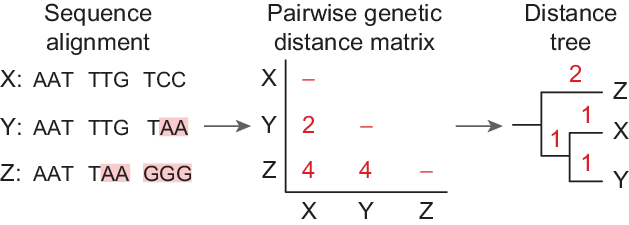
\includegraphics[width=.6\textwidth]{figures/Nj2.png}
\caption{Basic Graphic of what is going on in the Neighbor-joining algorithm and its Distance Matrix}
\end{figure}

\section{Methodology}

Now that we are familiar with all the components to this tree, we can finally begin our tree construction. 
As mentioned frequently, the taxa we will be working with is the Delta coronavirus variant. 
The inspiration for modeling this taxa was the recency bias of this global pandemic.
With the whole world being affected by this destructive virus, we are now beginning to see a wide array of mutations leading to different variants.
Tracking 112 different genomes, we looked specifically at the spike protein to construct our tree. 
Our intentions to construct the tree at the protein level was to significantly reduce the runtime for our computer program. 
With sequence alignment techniques varying at the DNA and protein level, we decided to try a novel approach using this Genetic algorithm at the protein interface.
Next we had it run through our Python program for a few minutes in which we were able to obtain the distance matrix. 
After doing so we fed our program to our MATLAB neighbor-joining algorithm where we are given our desired phylogenetic time tree. \emph{For those intersted and who might have missed it, we will be citing the Github for this research at the top }. 

\subsection{Our Time Tree}

\begin{figure}[H]
\centering
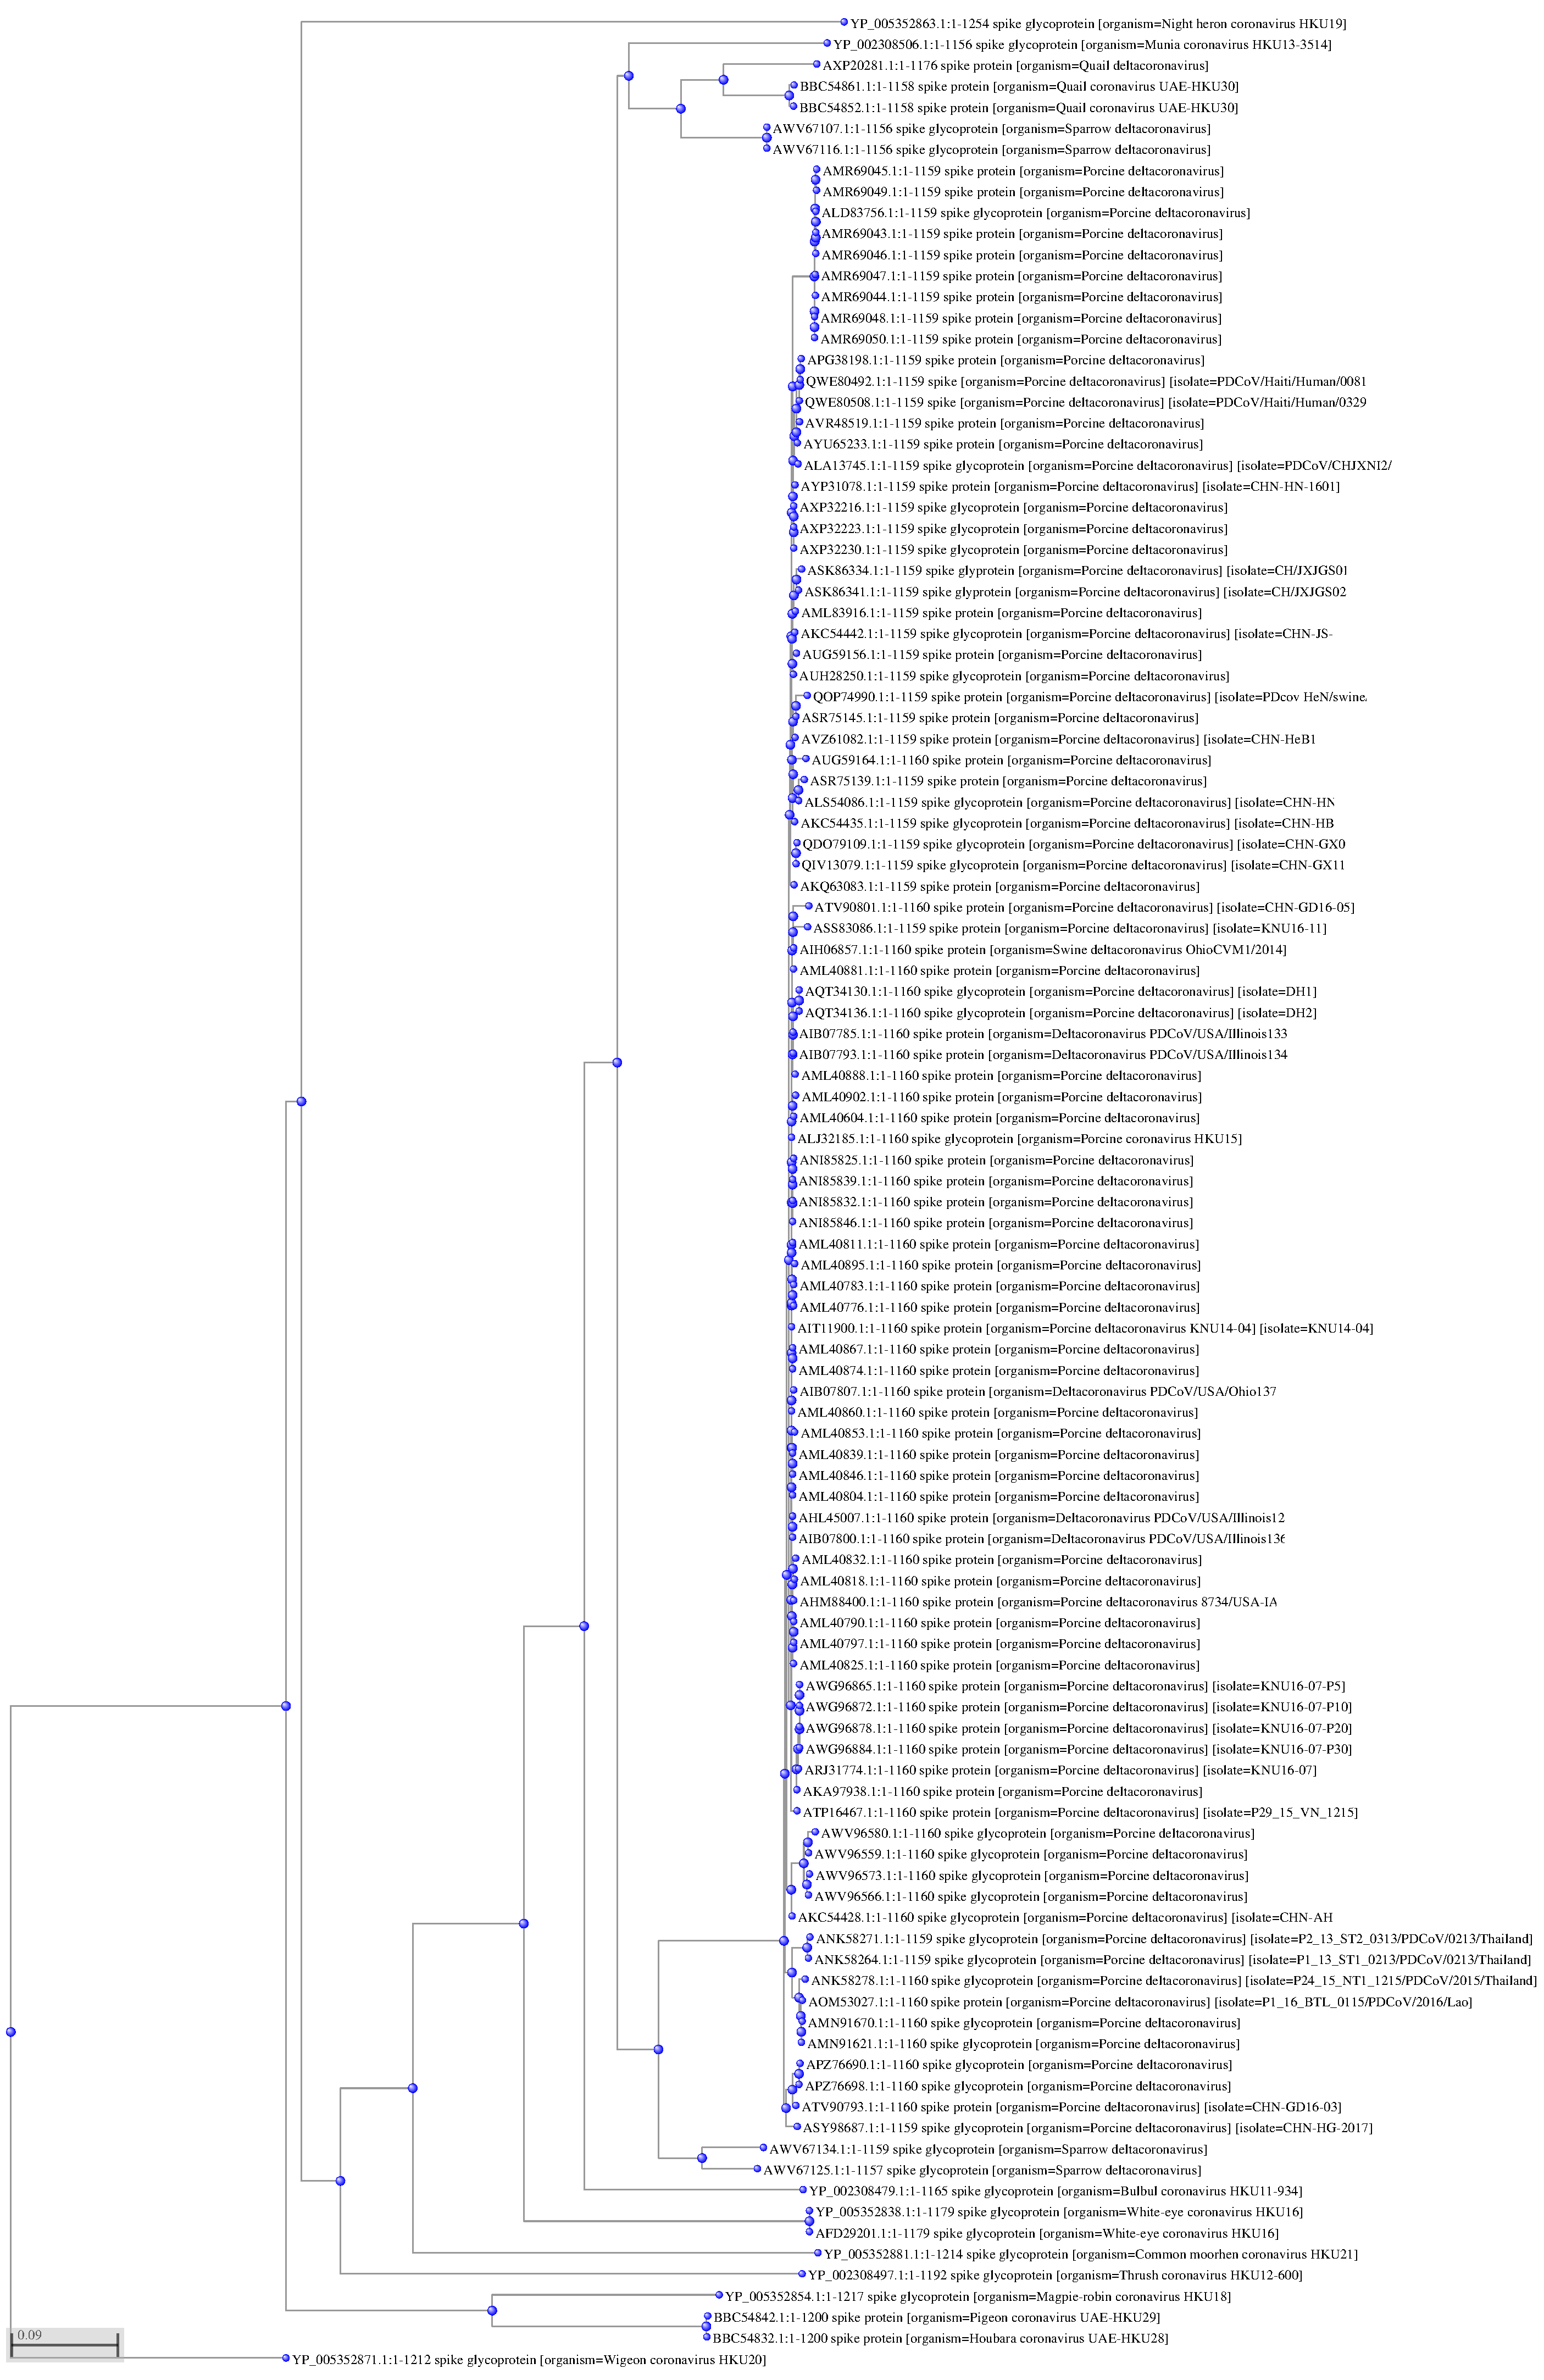
\includegraphics[width=.8\textwidth]{figures/tree-expanded.pdf}
\caption{Our 112 Species Time Phylogenetic Tree of the Deltacoronavirus variant. }
\end{figure}

After countless of hours of figuring out the best approaches to this problem, we have finally been able to produce a result.
The measure at the bottom is equivalent to 0.09 which is around 10.8 months. For every 0.1 in length it is equivalent to 1 year. 
To our surprise, the Delta variant has been around for much longer than we expected. Originating from the Middle East we ware able to observe some of our early findings of this longspread disease. 
While we did have some surprises, we can also see on the right hand side of the time tree all the recent chaos of the Delta variant spreading across species.

\subsection{Analysis and Findings}

In this section we will begin discussing our analysis, and findings of the SARS-CoV-2 Deltacoronavirus and how it spread amongst the 112 species sequences offered by the NCBI. As mentioned in previous sections, we are working with this taxa at the protein interface. Therefore we display below in our table how our data was read. Obviously the spike protein sequences are much longer in length but we decided to slice the first 25 characters for the selected Delta variant genomes.  

\begin{center}
\begin{tabular}{||c | c||} 
 \hline
 Genbank Code & Spike Protein (first 25 Amino Acids) \\
 \hline\hline
 HKU11-934 & MVKNVSKRSPIVLPQIQPPPLQLFI \\  
 \hline
 HKU12-600 & MAMNIAKRSPIVLPQIQPPPLQLFI \\ 
 \hline
 HKU13-3514 & MAKNKEKRSPIVLPELVPPPLQLFI \\
 \hline
 HKU16 & MGKNNPKRSPIVLPDPIPPPLQLFI \\
 \hline
 HKU17 & MAKNKSKRDAIALPENVPPPLQLFI \\
 \hline
 HKU18 & MAKNKEKRSPIALPEVVPPPLQLFI \\  
 \hline
 HKU19 & MGSKQVDHTCLTIPPNPSKTLALFI \\ 
 \hline
 HKU20 & MANKARPKGILVIPELSNNSSLLLL \\ 
 \hline
 HKU21 & MTKNSFDVGKVITLPKVIPPPLQLF \\ 
 \hline
 ... & .......				\\
\hline
 HKU15 & MAKNKSKRDAIALPENVPPPLQLFI \\ 
 \hline
\end{tabular}
\end{center}

In the above table, we are working specifically with the spike proteins which show significant signs of similarities. Within these similarities are slight differences which will all be accounted for when the Genetic Algorithm program took place. But through conducting some initial analysis the similar protein sequences will be joining together first when the neighbor-joining algorithm takes place, and we can begin to see some correlations between sequences. By no means is this a surprising observation considering we are working with the same species. But it is also interesting to see how these genomes have significantly mutated over time.  
   
Now we spend more time on the tree itself. With some of our genomes beginning at 2014, it makes intuitive sense as to why the graph is divided up as it is. With the majority of the tree falling between the 2019 to 2021 interval, it make aligns with the media and how this Coronavirus variant has spread within our "pandemic years". However within the trees there are also a few incorrect approximations. Because this Genetic algorithm only runs so many times, and is a stochastic machine learning algorithm, this randomness does make an appearance in the trees. With some genomes clearly labeled from 2014, 2016, 2018, they have been incorrectly placed towards where the majority of the data lies. There could be many reasons for these occurences. One of the reasons I could think of first off is our small sample size of genome data. The Spike protein coming from the SARS Delta Coronavirus is roughly 1,160 amino acids long. In retrospect the DNA sequence for one of these species is roughly 26865 nucletides long. Obviously if we were to run this experiment with DNA, our machine learning algorithm could pick up more insight based off the data it is presented. But as described one of of our main goals in this project was efficiency and computing time. Another possible reason for this error could be that the sequences are just very similar to one another. After running a more traditional multiple sequence alignment, we obtain the following results:

\begin{figure}[H]
\centering
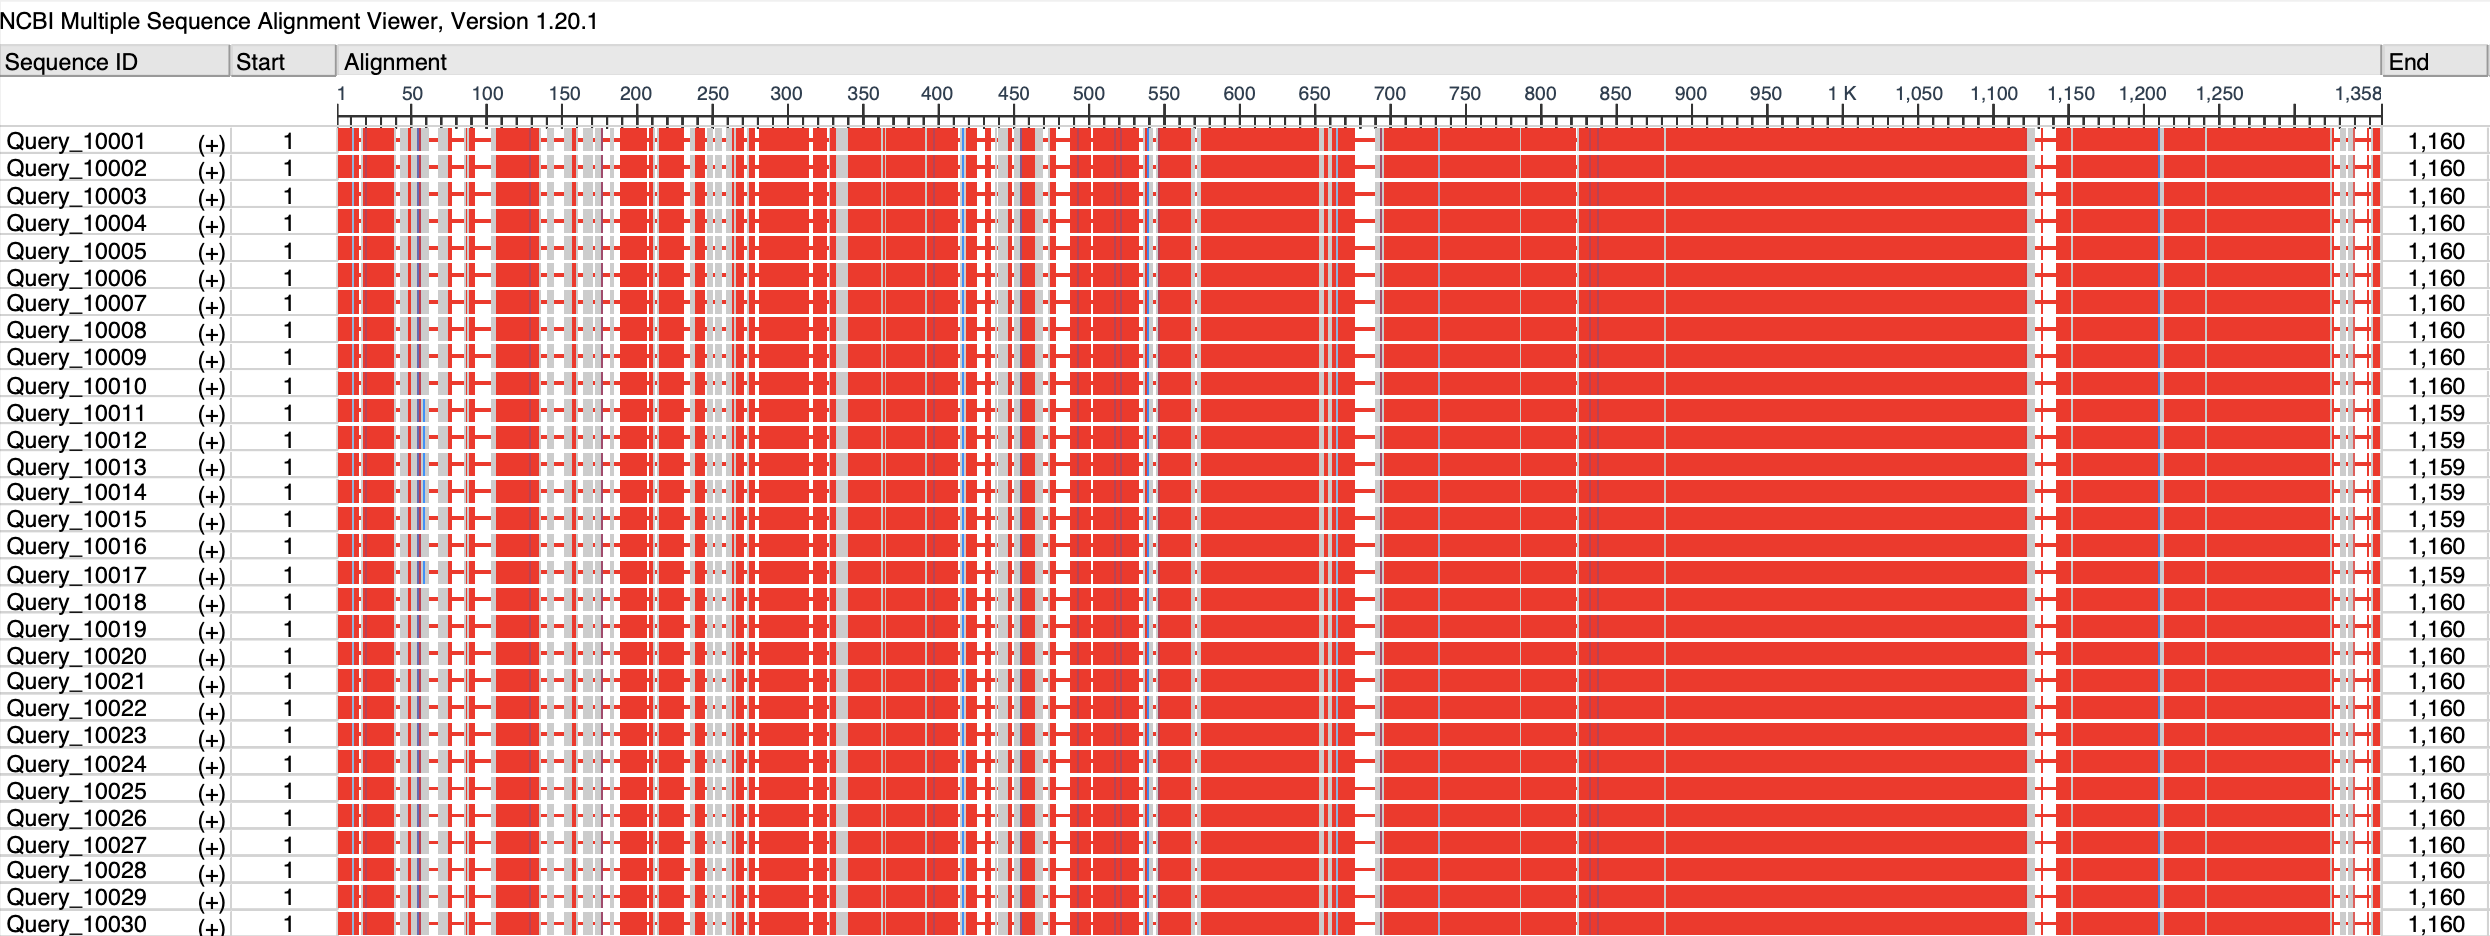
\includegraphics[width=.9\textwidth]{figures/sa2.png}
\caption{The first 30 genomes of a MSA.}
\end{figure}

\begin{figure}[H]
\centering
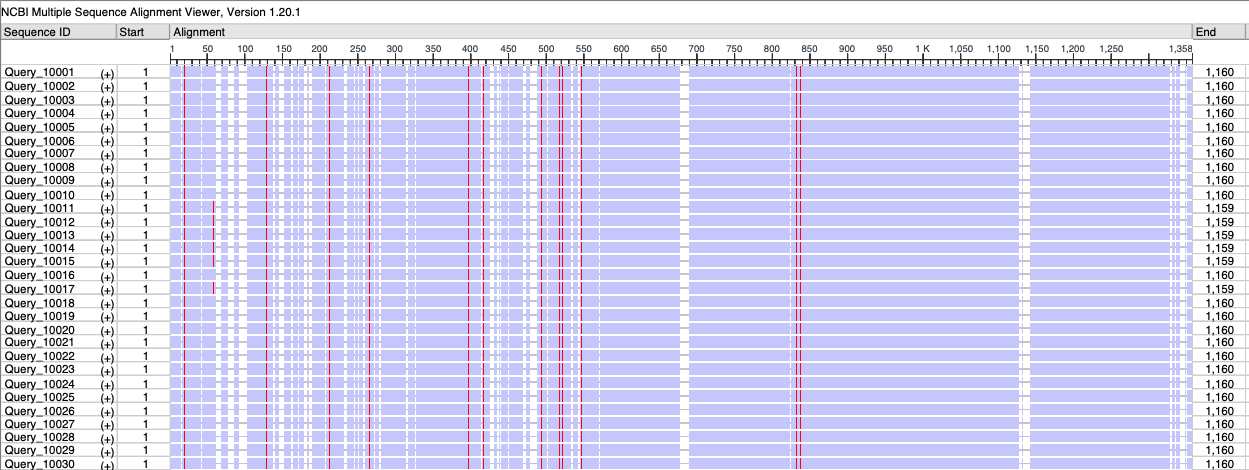
\includegraphics[width=.9\textwidth]{figures/sa1.png}
\caption{This visual makes it easy to see the similarities shown in \textbf{blue} and the dissimilarites shown in \textbf{red}}
\end{figure}

What I am trying to show is that throghout these genomes, they are very similar amongst each other. There are few instances where their amino acids are varying but for the most part this information is consistent. Once again this makes intutitive sense considering that these come from the same taxa. 

And lastly this algorithm is indeed stochastic. Even when we may have had a better tree construction in place, there is a small chance that the tree could have been eliminated by mutations. There is no way in this algorithm to preserve the best solutions because of the single point crossovers that must take place. Even with elitism incorperated, we only select the top 3 solutions to make it to the next generation. And because single point crossovers tend to produce better solutions, this behavior fluctuates. It is for these reasons that our tree is indeed a little faulty. However, overall the representation is true to what we were expecting. There are plenty of clusters appearing as we move from left to right in the dimension of time (\emph{t}). So this time tree I believe constructs a very abstract yet viable representation of a dynamical system. Given some moving variable t, our tree is bifurcating (spreading). Though this dynamical system resembles chaos moreso, with its unpredictable behaviors of when it will bifurcate, it still has many features which make it so. Though ambitious, we are content with the results we obtained from this research. Using the Genetic Algorithm as our main driver, we know the power that these machine learning algorithms can have in analyzing genomics data.  

\section{Conclusion}

Overall this research was quite the learning experience. Not only were we able to construct a fairly accurate phylogenetic time tree, but we were also able to solve a NP-hard bioinformatics problem. With data sciences becoming fairly impactful in biological research, we believe this is only the beginning for future advancements in bioinformatics. Slowly understanding genomics data, these phylogenetic trees can play much bigger roles in how we analyze spread of disease, and evolutionary relationships amongst different species. But with the SARS-CoV-2 pandemic with no end in sight, this field is crucial in understanding how much more dangerous this virus can potentially be. 

\section{Acknowledgement}

\emph{I want to thank the UCSC Applied Mathematics Department for supporting this project. Having spoken about this with Professor Marcella Gomez, and Vanessa Jonnson, I was finally able to find the right time and place to conduct this research. Before this iteration of this project went into full force, my intial proposal was deemed to simple, or too easy for any time of traction to come from this research. So I thank these professors for their educational criticism. I also want to thank Professor Daniele Venturi for teaching Applied Dynamical Systems. Before taking this course I did not think I would find the connections between my project at these dynamical systems. It is for this reason that I was able to complete this project.}


\begin{thebibliography}{15} 

\bibitem{Fliesler} Fliesler, N., \emph{Sturdier spikes may explain SARS-CoV-2 variants’ faster spread}, March 2021, Boston's Children Hospital, https://answers.childrenshospital.org/sars-cov-2-variants-spike, Accessed October 7.

\bibitem{Ahn} Ahn, C.W., Ramakrishna, R.S., \emph{Elitism-based compact genetic algorithms}, IEEE Transactions on Evolutionary Computation, Volume: 7, Issue: 4, Aug. 2003, Pages 367-385.  

\bibitem{Gammaitoni} Gammaitoni L., H$\"{a}$nggi P., Jung P., and Marchesoni F., \emph{Stochastic Resonance} Rev. Mod. Phys. 70, 223–288 (1998)

\bibitem{BB} 3Blue1Brown (n.d.) Neural Networks [What is backpropagation really doing? | Chapter 3, Deep learning]. Retrieved from https://www.youtube.com/playlist?list=PLZHQObOWTQDNU6R1\_67000Dx\_ZCJB-3pi

\bibitem{Hardesty} Hardesty, L., \emph{Explained: P vs. NP, The most notorious problem in theoretical computer science remains open, but the attempts to solve it have led to profound insights.}, October 2009, https://news.mit.edu/2009/explainer-pnp, Accessed October 11.

\bibitem{Ecology} \emph{Bifurcating Trees}, Ecology Center, https://www.ecologycenter.us/genetic-diversity/bifurcating-trees.html, Acessed October 14.

\bibitem{Clade} \emph{Understanding Evolution: your one-stop source for information on evolution}, The Tree Room, https://evolution.berkeley.edu/evolibrary/article/0\_0\_0/evotrees\_intro, Accessed October 14. 


\end{thebibliography}


